\documentclass[12pt]{article}

\usepackage[margin=2cm]{geometry}
\usepackage{amsmath}
\usepackage{multicol}
\usepackage{nopageno}
\usepackage{SIunits}
\usepackage{graphicx}
\usepackage{enumerate}
\usepackage{enumitem}
%\usepackage{mathabx}
\usepackage{wasysym}


% for making bond drawings
\usepackage{chemfig}
% Global bond settings
\setchemfig{
  atom sep=18pt,               % fixed bond length
  double bond sep=2pt,       % spacing between the two bars
  bond style={line width=0.8pt}
}


% for centering figures on page while in an enumerated/itemized list:
\usepackage{changepage} % in the preamble
\makeatletter
\newenvironment{centerinpage}
  {%
    \par\noindent
    \hspace*{-\@totalleftmargin}% back to page margin (covers all nested list indents)
    \begin{minipage}{\textwidth}% fixed to page width (ignores widened \linewidth)
      \centering
  }
  {%
    \end{minipage}\par
  }
\makeatother

%%%%%%%%%%%%%%%%%%%%%%%%%%%%%%%%%%%%%%%%%%%%%%%%%%%%%
% For putting links in the document (both to sections and hyperlinks)
\usepackage{hyperref}
\usepackage{url}
\hypersetup{
    colorlinks=true,     % false: boxed links; true: colored links
    linkcolor=red,       % color of internal links
    citecolor=blue,      % color of links to bibliography
    filecolor=blue,      % color of file links
    urlcolor=blue        % color of external links
}
% below, use \url{http://www.nytimes.com} (they will be urlcolor)
%%%%%%%%%%%%%%%%%%%%%%%%%%%%%%%%%%%%%%%%%%%%%%%%%%%%%


%%%%%%%%%%%%%%%%%%%%%%%%%%%%%%%%%%%%%%%%%%%%%%%%%%%%%
% for the events page boxes

% boxed regions
\usepackage{tcolorbox}
\tcbuselibrary{skins,breakable}

% fonts & spacing
\usepackage{lmodern}
\usepackage{microtype}
\usepackage{calc}


% small helper macros (adjust these)
\newcommand{\boxheight}{4.2cm}   % height for each event box
\newcommand{\boxfont}{\scriptsize} % change to \tiny or \footnotesize as desired
\newcommand{\linelen}{0.95\linewidth} % timeline line length

%%%%%%%%%%%%%%%%%%%%%%%%%%%%%%%%%%%%%%%%%%%%%%%%%%%%%
\newcommand{\rmd}{\ensuremath{{\rm d}}}
%\newcommand{\vv}[1]{\ensuremath{\vec{#1}}}
\newcommand{\vv}[1]{\ensuremath{\mathbf{#1}}}
\newcommand{\ee}[1]{\ensuremath{\mathbf{e}_{#1}}}
%%%%%%%%%%%%%%%%%%%%%%%%%%%%%%%%%%%%%%%%%%%%%%%%%%%%%



\begin{document}

\begin{center}
{\Large Milankovitch Cycles}
\end{center}
%%%%%%%%%%%%%%%%%%%%%%%%%%%%%%%%%%%%%%%%%%%%%%%%
%%%%%%%%%%%%%      overview         %%%%%%%%%%%%%%%%%%%%%
%%%%%%%%%%%%%%%%%%%%%%%%%%%%%%%%%%%%%%%%%%%%%%%%


%
%\newpage
%%%%%%%%%%%%%%%%%%%%%%%%%%%%%%%%%%%%%%%%%%%%%%%%
%%%%%%%%%%%%%      questions         %%%%%%%%%%%%%%%%%%%%%
%%%%%%%%%%%%%%%%%%%%%%%%%%%%%%%%%%%%%%%%%%%%%%%%

\begin{enumerate}

\item  The {\bf Milankovitch cycles} are periodic oscillations of solar irradiance --- recall that the ``{\bf Solar Constant}'' is $S=\unit{1360}{\joule/\second/\meter^2}$; we are talking about {\em variations of this number} over time --- due to changes in the Earth's {\bf revolution} around the Sun and {\bf rotation} on its axis.
	%
	\begin{enumerate}
	\item The cycles are due to three primary effects:
		%
		\begin{itemize}
		\item Changes in the {\bf eccentricity} of the Earth's orbit around the Sun.
		\item Changes in the {\bf obliquity} of the Earth's rotational axis.
		\item Changes due to the {\bf precession} of the Earth's rotational axis.
		\end{itemize}
		%
	Let's identify in your own words what these things mean.  Consider the information in: the class slides this week; Section 7.4 of our Dessler textbook; the brief NASA explanation and videos linked\footnote{The NASA page is: {\small \url{https://science.nasa.gov/science-research/earth-science/milankovitch-orbital-cycles-and-their-role-in-earths-climate/}}.} on Blackboard (under Class Slides); the beginning of Chapter 7 of the Mathez textbook (also linked on Blackboard.  Then:
		%
		\begin{enumerate}[label=(\roman*)]
		\item Define these terms using your own words and pictures: eccentricty, obliquity, and precession. 
		\item Describe the three changes in these quantites (or changes associated to these quantities) as the Earth revolves and rotates. 
		\item Explain how each type of change would alter the solar irradiation of Earth (e.g., how would it change the timing and length of seasons in one hemisphere or another).
		\end{enumerate}
		%
	\item From the resources above, identify the {\bf period} associated to each of the three Milankovitch cycle changes (i.e., the amount of time for each to complete one full cycle).  Then, using graph paper (landscape orientation), draw three rows of graphs, where the horizontal axis is time and the scale is set to be the same for each.  Choose that horizontal scale so that you can see at least two cycles of each (so at least {\em twice the longest period}).  Then draw a sinusoidal curve\footnote{You will see in your readings and in the graphs below, that these periods are approximate. None of these effects are exactly described by a sinusoidal curve with a fixed period.}  for each type of oscillation such that it matches the periods that you identified.
	\item Let's consider a ``toy model'' of oscillations for a moment.  Imagine that the three different oscillations have periods of two, three, and five years respectively.  If they were all to start at their peak values on the sinusoid (e.g., the orbital configuration representing maximal solar irradiance), after how much time would they arrive back at the same point, all at their peak values again simultaneously? Explain your answer in words, equations, and or pictures. \\[6pt] 	 [{\bf Bonus:} What is the general way that one can solve this problem, and is there always a solution?  What is the answer for the Milankovitch cycles, i.e., how much time for all three types of cycles to return to their maximum values together? ]	
	\end{enumerate}

\newpage

\item {\bf Paleotemperature records} Figure \ref{fig:milankovitch-wiki} shows the Milankovitch oscillations for the past 800,000 years and coming 800,00  years.
	%
	\begin{enumerate}
	\item Using a ruler, the timescale shown on the horizontal axis of Figure \ref{fig:milankovitch-wiki}, and the information given in the figure caption, find the three periods you identified from question 1. For example, use a bar to indicate a time range containing an integer number (5--10?) of each cycle.
	%\item The fourth row indicates the assumed net effect of the Milankovitch cycles: solar radiation at 65N latitude.  Why would northern hemisphere insolation be impor
	\item The prior time period --- the past million years --- is called the ``ice ages'' because of the cycles of ``glacial'' and ``interglacial'' periods.  Identify on the figure our current interglacial period, and all prior glacial/interglacial periods.  
	\item It is said that this span of time is characterized by a 100 ky periodicity.  Do you see any evidence for that in the temperature (proxy) record? Explain.  What might cause the 100 ky periodicity?  Do you see any connection between the Milankovitch cycles and the periodicity in the temperature record?
	\item In Figure \ref{fig:petit-vostok-milankovitch} we see a more zoomed in display of the past 400,000 years, together with the Milankovitch summary result (insolation at 65N latitude), taken from the original 1999 Nature paper that reported the Vostok ice core results.  The authors have made some links between the temperature proxy data and the Milankovitch curve.  Looking at this figure and reading through the original 1999 paper (available on blackboard in the Class Slides section), comment on these connections.  What do the authors claim to be the connection here?
	\end{enumerate}

\end{enumerate}

\newpage

%%%%%%%%%%%%%%%%%%%%%%%%%%%%%%
%\mbox{}
%\newpage
%%%%%%%%%%%%%%%%%%%%%%%%%%%%%%

%%%%%%%%%%%%%%%%%%%%%%%%%%%%%%%%%%%%%%%%%%%%%%%%%%%%
%%%%%%%%%%               milankovitch wikimedai            %%%%%%%%%%%%%
%%%%%%%%%%%%%%%%%%%%%%%%%%%%%%%%%%%%%%%%%%%%%%%%%%%%

\begin{figure}
\centering
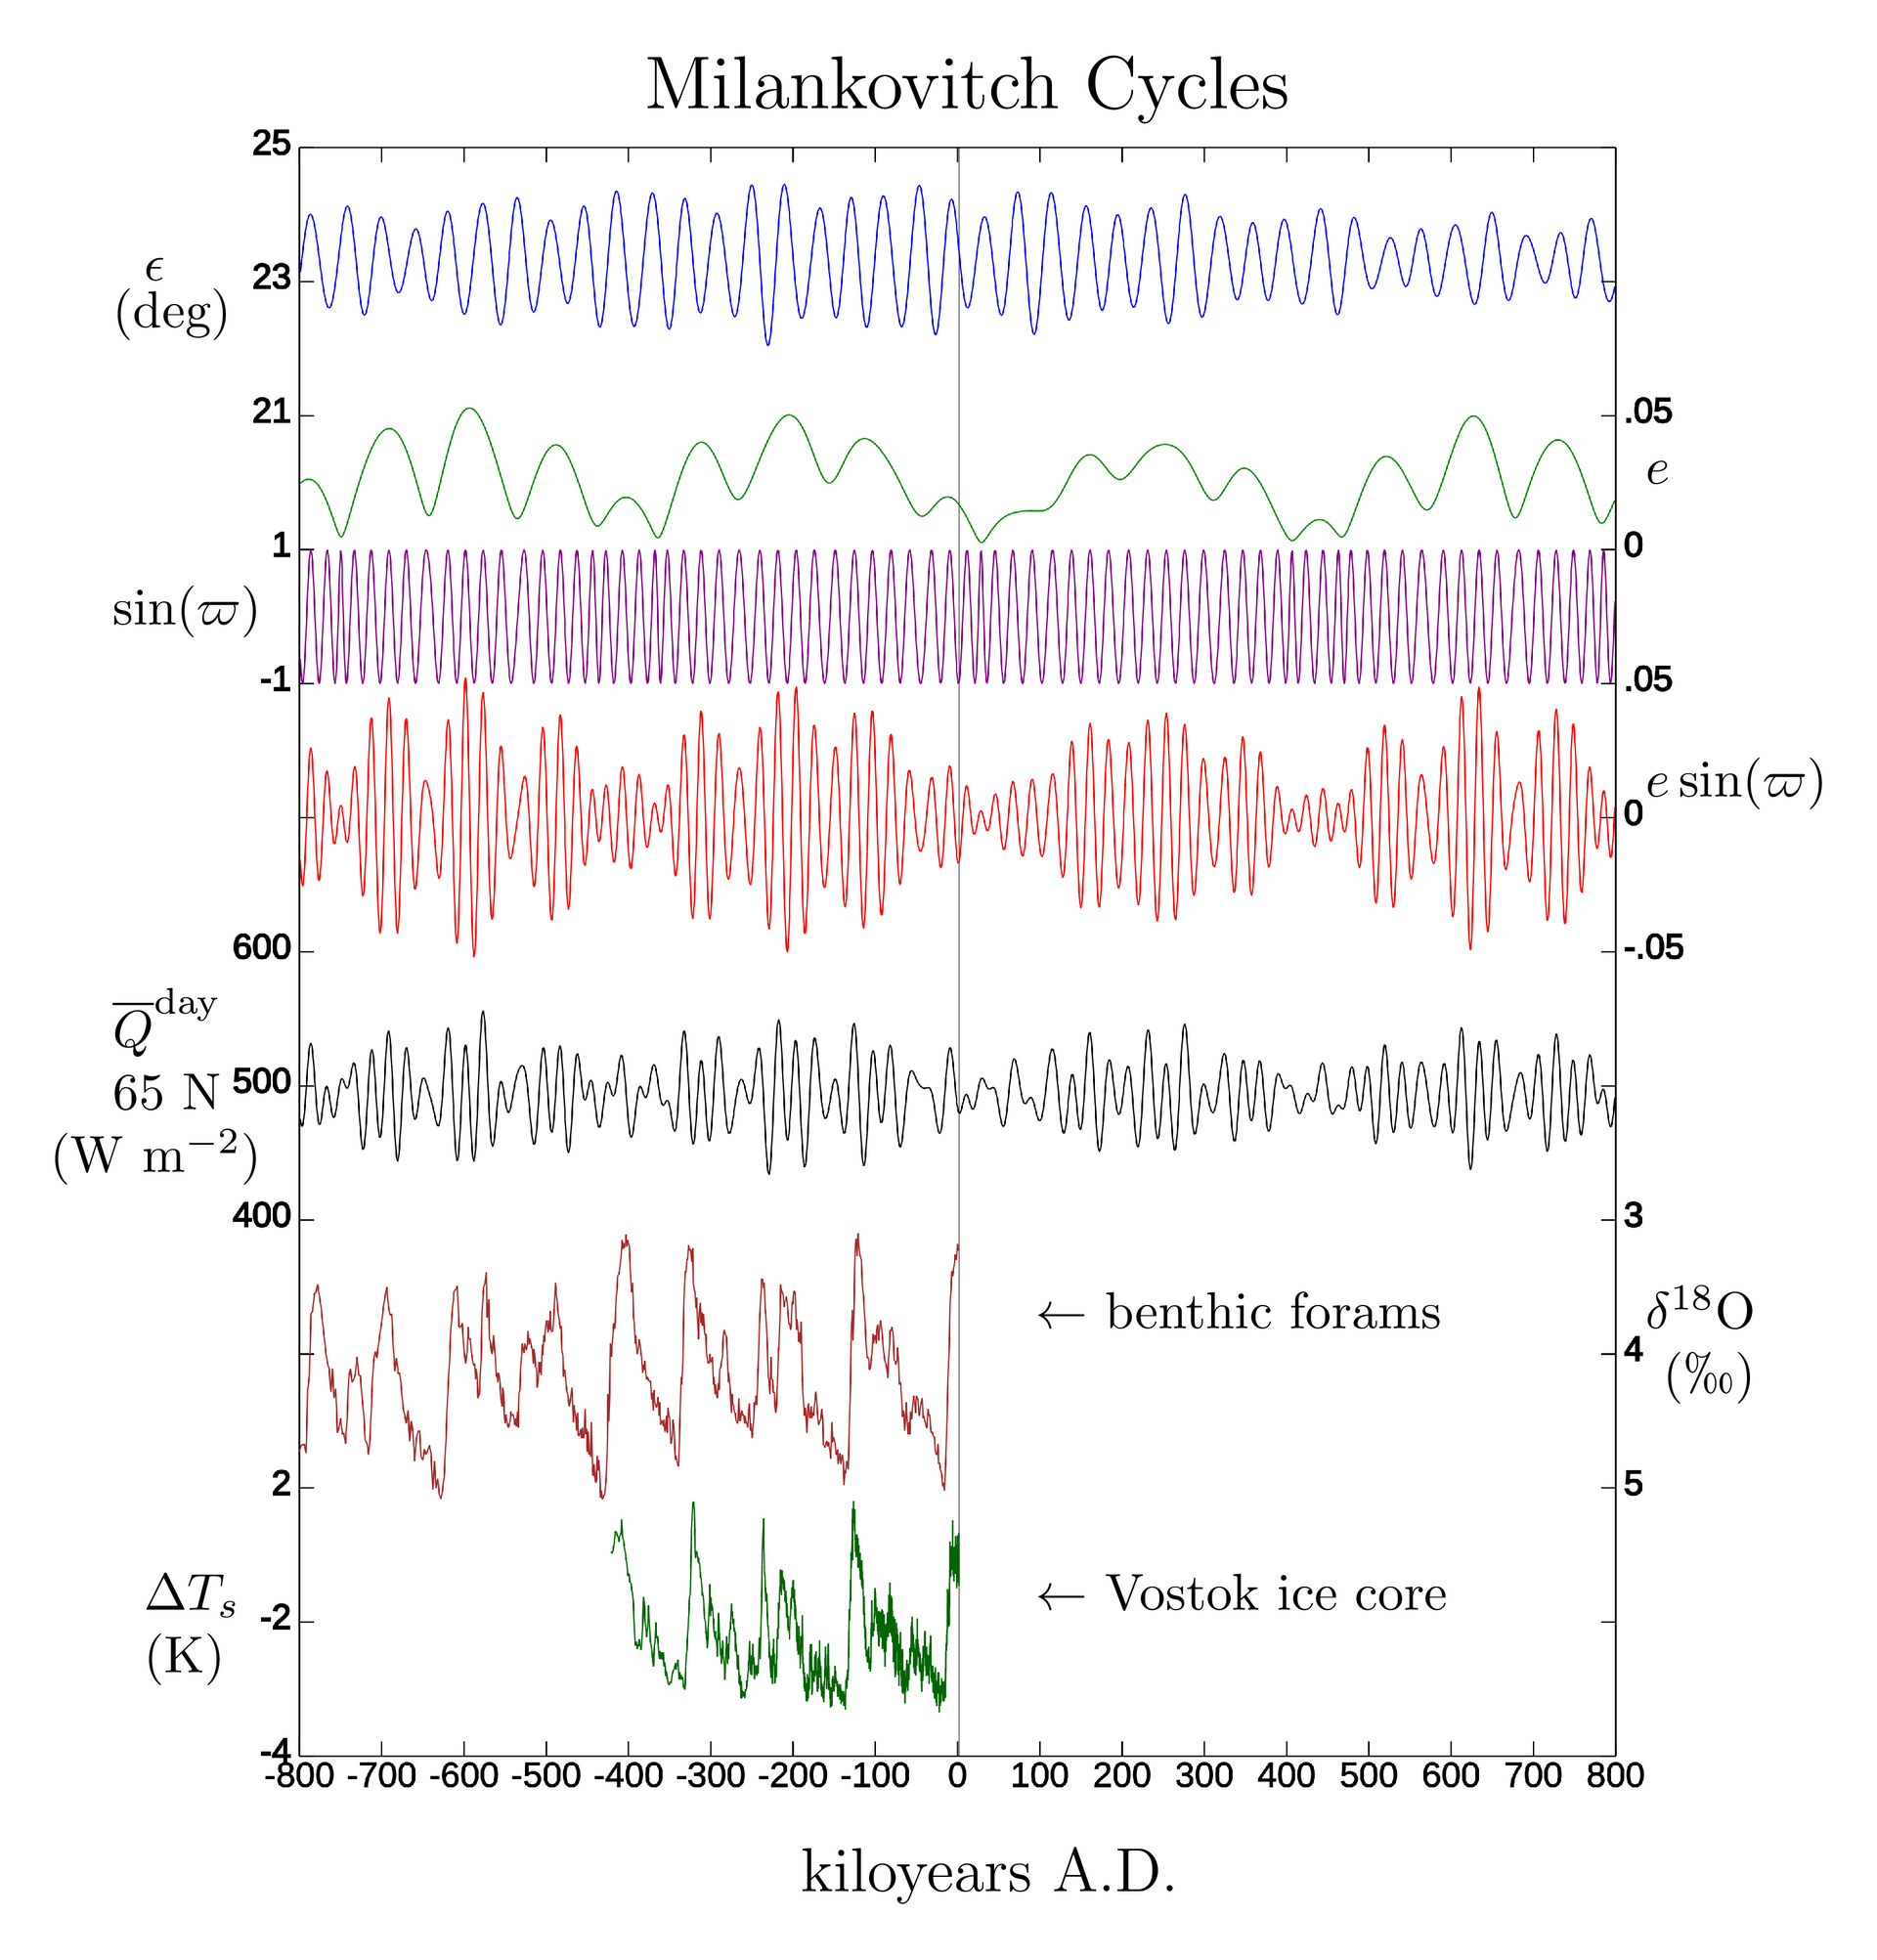
\includegraphics[width=\textwidth]{images/milankovitch_wikimedia-incredio.png}

\caption{ \label{fig:milankovitch-wiki}
{\bf First row:} Obliquity angle, $\epsilon$, over time. {\bf Second row:} Eccentricity, $e$, over time. {\bf Third row:} Axis precession, $\sin \varpi$, over time. {\bf Fourth row:} The ``precession index'' (eccentricity times precession), $e \sin \varpi$, over time. {\bf Fifth row:} Estimated solar radiation at 65N latitude --- found by multiplying the effect of obliquity and the precession index. {\bf Sixth row:} Paleotemperature proxy from the incorporation of oxygen isotopes in shells of marine organisms. {\bf Seventh row:} Paleotemperature (anomaly) estimates from Antartic ice cores, from direct measurements of oxygen isotopes in trapped gas.  [From Wikipedia by user incredio]
}
\end{figure}

\newpage

\begin{figure}
\centering
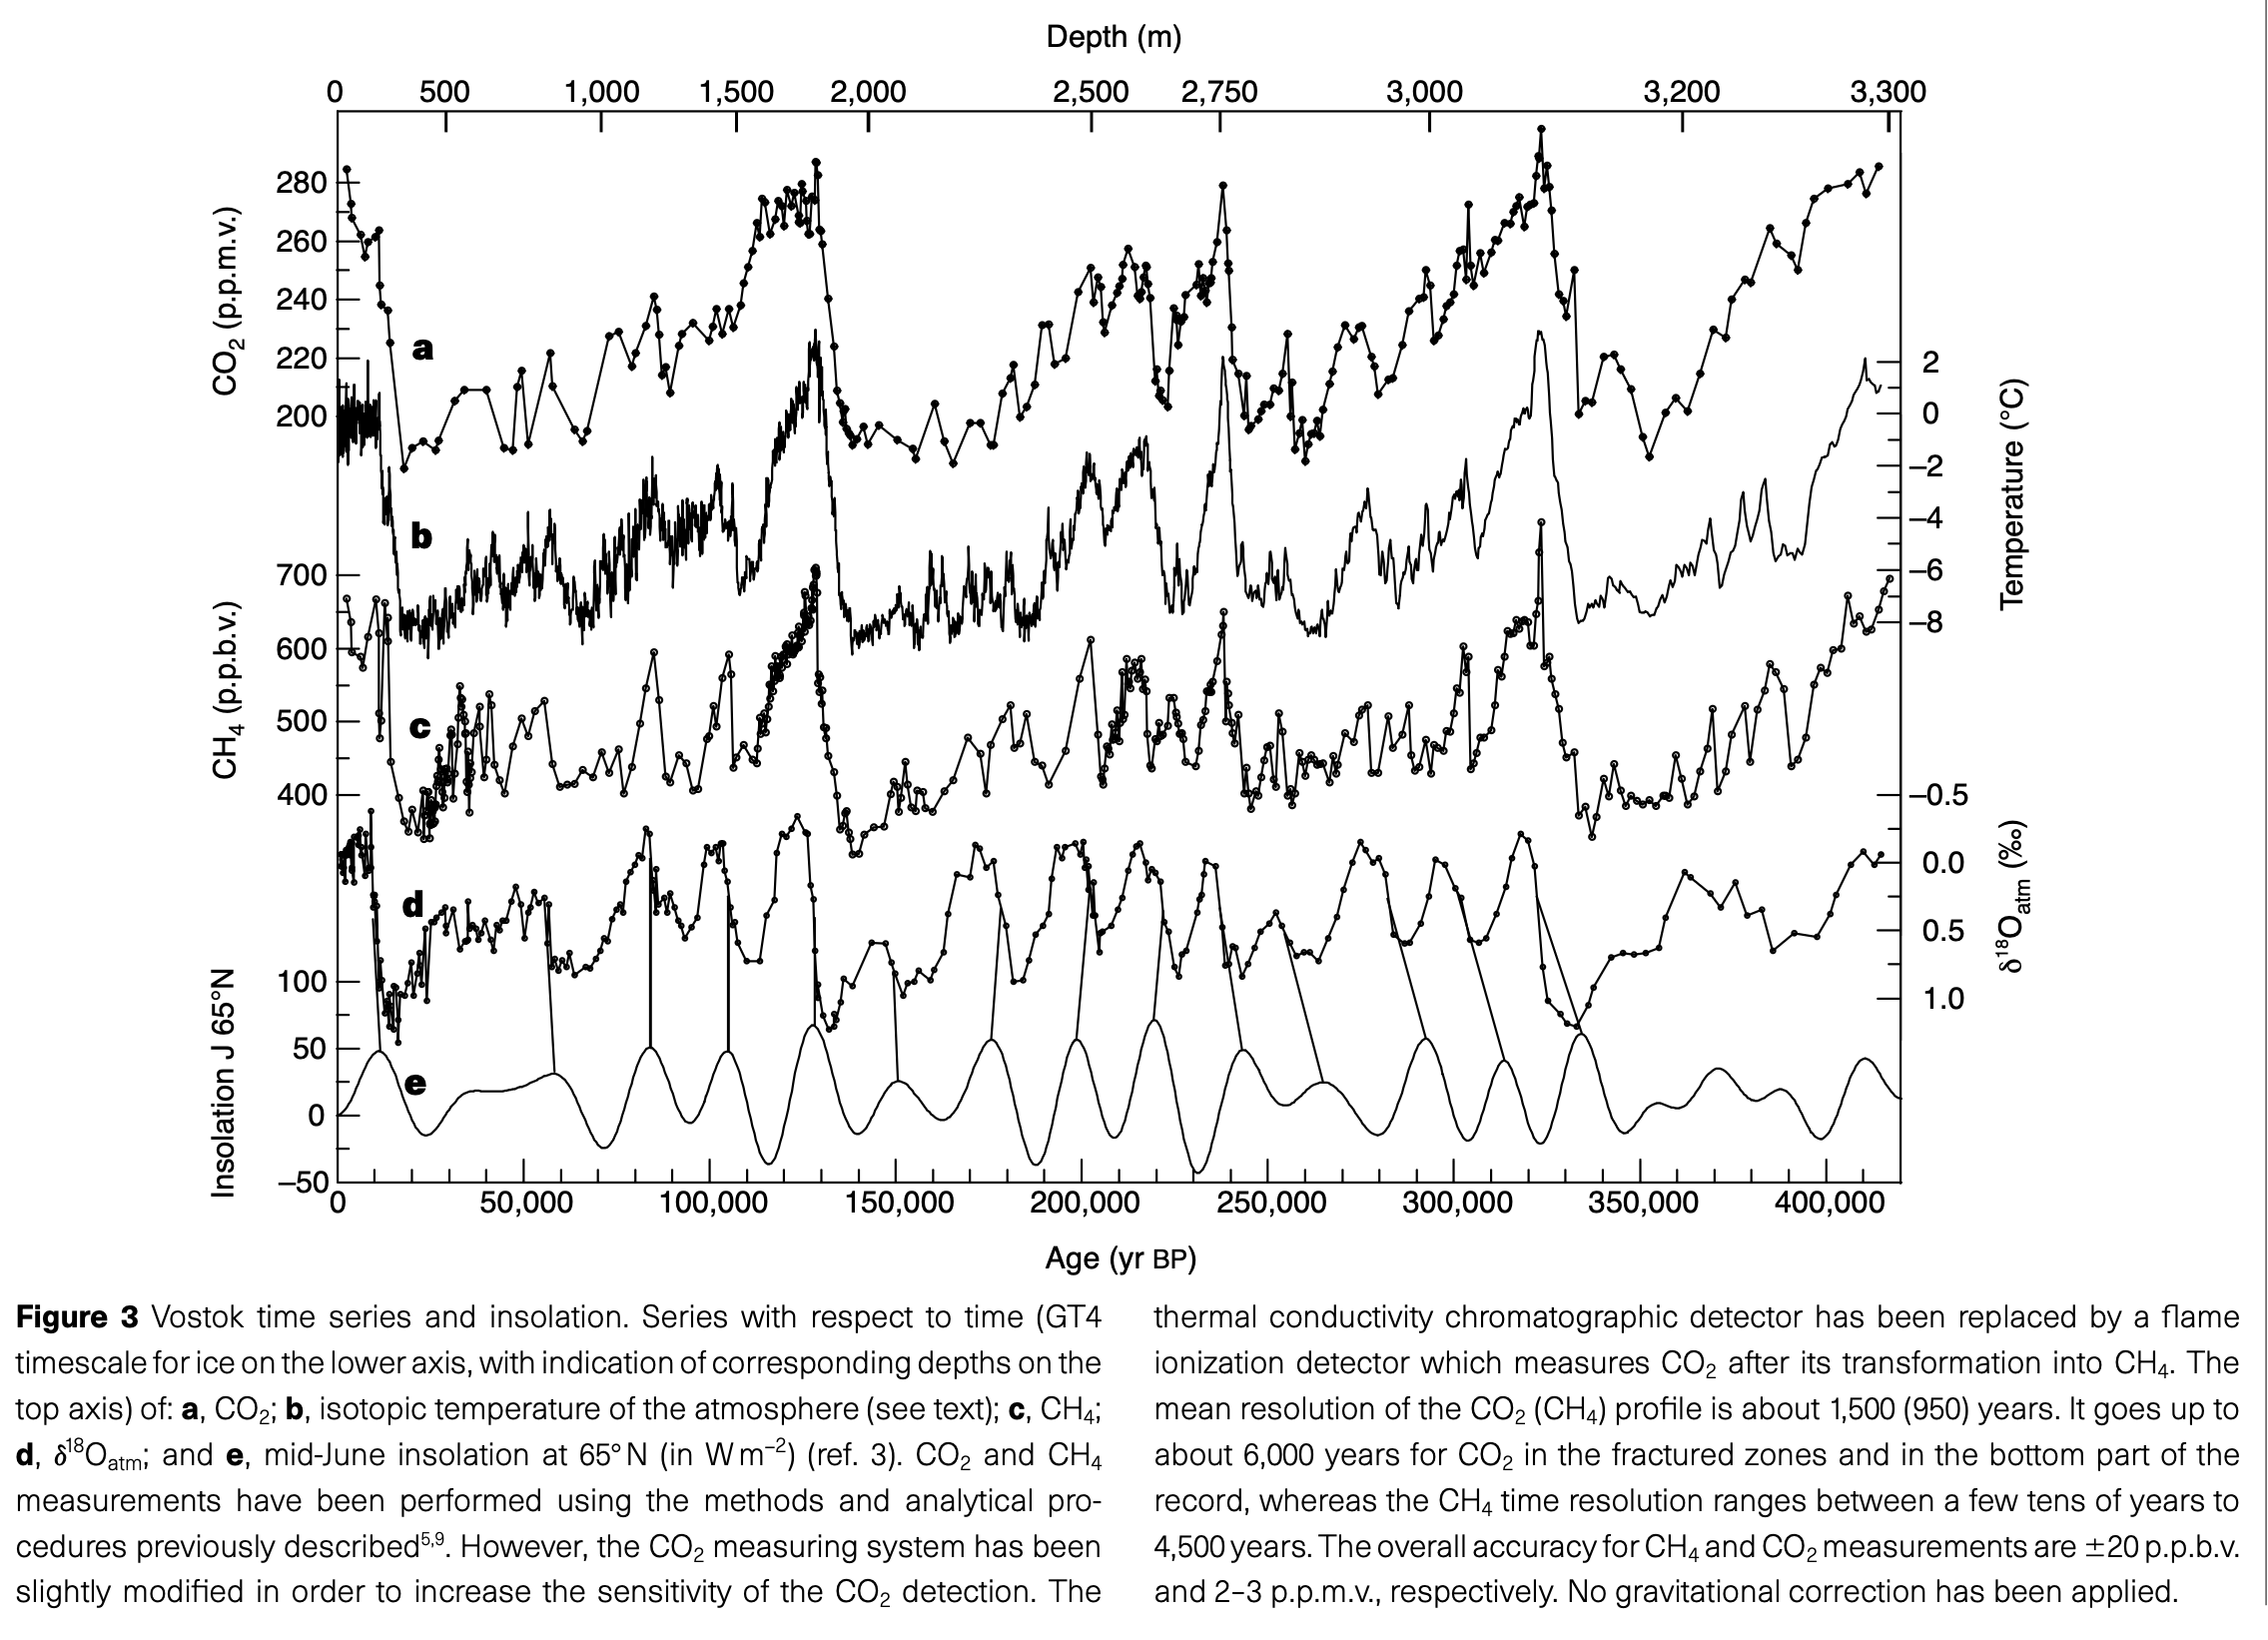
\includegraphics[width=\textheight, angle=90]{images/petit-etal_fig3.png}

\caption{ \label{fig:petit-vostok-milankovitch}
[Figure 3 from  Petit et.\ al.\ (Nature 1999)]]
}
\end{figure}

%%%%%%%%%%%%%%%%%%%%%%%%%%%%%%%%%%%%%%%%%%%%%%%%%%%%
%%%%%%%%%%                                  References                                %%%%%%%%%%%%%%%%
%%%%%%%%%%%%%%%%%%%%%%%%%%%%%%%%%%%%%%%%%%%%%%%%%%%%
%\noindent {\bf Data Sources}: 



\end{document}
